\appendix
\chapter{Anhang}
\section{Graph-Datenbanken - Grundlegende technologische Aspekte}
\section{Graph-Datenbanken und -Frameworks - Ausgewählte Systeme}
\begin{figure}[H]

    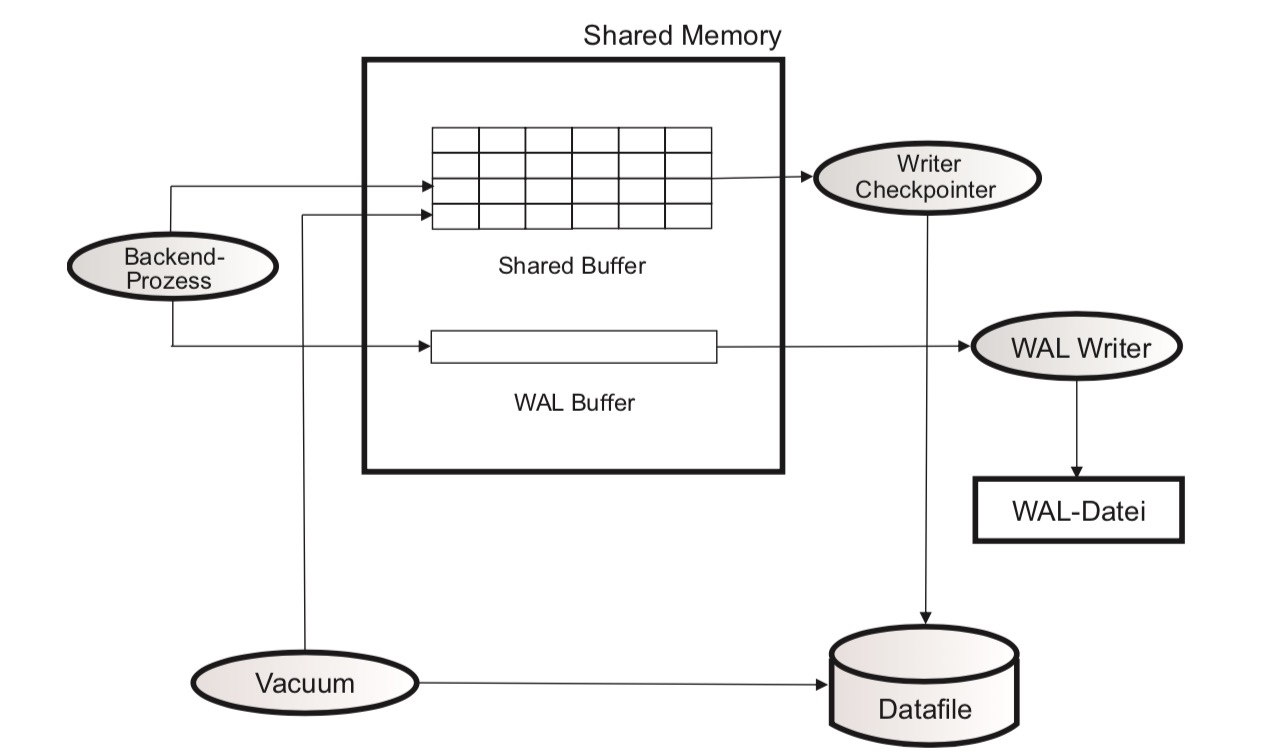
\includegraphics[width = \linewidth]{images/postgresArchitektur.jpg}
    \caption{Postgres Architektur}
    \label{Postgres Architektur}

\end{figure}
\section{Graph-Datenbanken im praktischen Einsatz: OLTP}
\lstsetsql
\begin{lstlisting}[language=SQL,caption=CSV Input,frame=single, label={copy}]
    \copy Beitraege
    FROM './data/Beitraege.csv' DELIMITER ',' CSV HEADER;
\end{lstlisting}

\begin{lstlisting}[language=SQL,caption=Anlegen der Tabelle facebook-profiles,frame=single, label={facebookProfiles}]
    create TABLE IF NOT EXISTS profiles_facebook(
        ID INTEGER PRIMARY KEY,
        first VARCHAR(50),
        last VARCHAR(50),
        gender GENDER,
        birth DATE,
        country VARCHAR(50)
    );
\end{lstlisting}

\begin{lstlisting}[language=SQL,caption=Anlegen der Tabelle facebook-relation,frame=single, label={relationFacebook}]
    CREATE TABLE IF NOT EXISTS relation_facebook(
        src INTEGER REFERENCES profiles_facebook(ID),
        dst INTEGER REFERENCES profiles_facebook(ID),
        type VARCHAR(50),
        date DATE
    );
\end{lstlisting}

\begin{lstlisting}[language=SQL,caption=Hinzufügen von Fremdschlüsseln,frame=single, label={foreignKey}]
    \copy profiles_facebook_tmp(first,last,gender,birth,country) FROM '/data/WS2018/facebook-profiles' DELIMITER ',' CSV HEADER;
    INSERT INTO profiles_facebook (ID, first, last, gender, birth, country)
    SELECT ID-1, first, last, gender, birth, country from profiles_facebook_tmp;
\end{lstlisting}

\begin{lstlisting}[language=SQL,caption=Erstellen von partitionierten Tabellen mit Index facebook,frame=single, label={parttableindexfacebook}]
    CREATE TABLE IF NOT EXISTS relation_facebook_partitioned(
        src INTEGER REFERENCES profiles_facebook(ID),
        dst INTEGER REFERENCES profiles_facebook(ID),
        type VARCHAR(50),
        date DATE
    )PARTITION BY RANGE(src);

    CREATE INDEX fb_part_src ON relation_facebook_partitioned (src);
    CREATE INDEX fb_part_dst ON relation_facebook_partitioned (dst);

    CREATE TABLE relation_facebook_partitioned_0 PARTITION OF relation_facebook_partitioned
    FOR VALUES FROM (0) TO (23000);
    CREATE TABLE relation_facebook_partitioned_1 PARTITION OF relation_facebook_partitioned
    FOR VALUES FROM (23000) TO (46000);
    CREATE TABLE relation_facebook_partitioned_2 PARTITION OF relation_facebook_partitioned
    FOR VALUES FROM (46000) TO (69000);
    CREATE TABLE relation_facebook_partitioned_3 PARTITION OF relation_facebook_partitioned
    FOR VALUES FROM (69000) TO (92000);
\end{lstlisting}

\begin{lstlisting}[language=SQL,caption=Erstellen von Indexen auf relation Tabelle facebook,frame=single, label={indexfacebook}]
    CREATE INDEX fb_dst ON relation_facebook_with_index (dst);
    CREATE INDEX fb_src ON relation_facebook_with_index (src);
\end{lstlisting}

\begin{lstlisting}[language=SQL,caption=Erstellen von partitionierten Tabellen mit Index youtube,frame=single, label={parttableindexyoutube}]
    CREATE TABLE IF NOT EXISTS relation_youtube_partitioned(
        src INTEGER REFERENCES profiles_youtube(ID),
        dst INTEGER REFERENCES profiles_youtube(ID),
        type VARCHAR(50),
        date DATE
    )PARTITION BY RANGE(src);

    CREATE INDEX yt_part_src ON relation_youtube_partitioned (src);
    CREATE INDEX yt_part_dst ON relation_youtube_partitioned (dst);

    CREATE TABLE relation_youtube_partitioned_0 PARTITION OF relation_youtube_partitioned
    FOR VALUES FROM (0) TO (800000);
    CREATE TABLE relation_youtube_partitioned_1 PARTITION OF relation_youtube_partitioned
    FOR VALUES FROM (800001) TO (1600000);
    CREATE TABLE relation_youtube_partitioned_2 PARTITION OF relation_youtube_partitioned
    FOR VALUES FROM (1600001) TO (2400000);
    CREATE TABLE relation_youtube_partitioned_3 PARTITION OF relation_youtube_partitioned
    FOR VALUES FROM (2400001) TO (3200000);
\end{lstlisting}

\begin{lstlisting}[language=SQL,caption=Erstellen von Indexen auf relation Tabelle youtube,frame=single, label={indexyoutube}]
    CREATE INDEX yt_dst ON relation_youtube_with_index (dst);
    CREATE INDEX yt_src ON relation_youtube_with_index (src);
\end{lstlisting}

\begin{lstlisting}[language=SQL,caption=Erstellen von partitionierten Tabellen mit Index livejournal,frame=single, label={parttableindexlivejournal}]
    CREATE TABLE IF NOT EXISTS relation_livejournal_partitioned(
        src INTEGER REFERENCES profiles_livejournal(ID),
        dst INTEGER REFERENCES profiles_livejournal(ID),
        type VARCHAR(50),
        date DATE
    )PARTITION BY RANGE(src);

    CREATE INDEX lj_part_src ON relation_livejournal_partitioned (src);
    CREATE INDEX lj_part_dst ON relation_livejournal_partitioned (dst);

    CREATE TABLE relation_livejournal_partitioned_0 PARTITION OF relation_livejournal_partitioned
    FOR VALUES FROM (0) TO (10000000);
    CREATE TABLE relation_livejournal_partitioned_1 PARTITION OF relation_livejournal_partitioned
    FOR VALUES FROM (10000000) TO (20000000);
    CREATE TABLE relation_livejournal_partitioned_2 PARTITION OF relation_livejournal_partitioned
    FOR VALUES FROM (20000000) TO (30000000);
    CREATE TABLE relation_livejournal_partitioned_3 PARTITION OF relation_livejournal_partitioned
    FOR VALUES FROM (30000000) TO (40000000);
\end{lstlisting}

\begin{lstlisting}[language=SQL,caption=Erstellen von Indexen auf relation Tabelle livejournal,frame=single, label={indexlivejournal}]
    CREATE INDEX lj_src ON relation_livejournal_with_index (src);
    CREATE INDEX lj_dst ON relation_livejournal_with_index (dst);
\end{lstlisting}

\begin{lstlisting}[language=SQL,caption=Erstellen von partitionierten Tabellen mit Index epinion,frame=single, label={parttableindexepinion}]
    CREATE TABLE IF NOT EXISTS relation_epinions_partitioned(
        src INTEGER REFERENCES profiles_epinions(ID),
        dst INTEGER REFERENCES profiles_epinions(ID),
        type VARCHAR(50),
        date DATE
    )PARTITION BY RANGE(src);

    CREATE INDEX ep_part_src ON relation_epinions_partitioned (src);
    CREATE INDEX ep_part_dst ON relation_epinions_partitioned (dst);

    CREATE TABLE relation_epinions_partitioned_0 PARTITION OF relation_epinions_partitioned
    FOR VALUES FROM (0) TO (102000);
    CREATE TABLE relation_epinions_partitioned_1 PARTITION OF relation_epinions_partitioned
    FOR VALUES FROM (102000) TO (204000);
    CREATE TABLE relation_epinions_partitioned_2 PARTITION OF relation_epinions_partitioned
    FOR VALUES FROM (204000) TO (306000);
    CREATE TABLE relation_epinions_partitioned_3 PARTITION OF relation_epinions_partitioned
    FOR VALUES FROM (306000) TO (408000);
\end{lstlisting}

\begin{lstlisting}[language=SQL,caption=Erstellen von Indexen auf relation Tabelle epinion,frame=single, label={indexepinion}]
    CREATE INDEX ep_dst ON relation_epinions_with_index (dst);
    CREATE INDEX ep_src ON relation_epinions_with_index (src);
\end{lstlisting}

\begin{lstlisting}[language=SQL,caption=Erstellen von partitionierten Tabellen mit wikivote epinion,frame=single, label={parttableindexwikivote}]
    CREATE TABLE IF NOT EXISTS relation_wiki_vote_partitioned(
        src INTEGER REFERENCES profiles_wiki_vote(ID),
        dst INTEGER REFERENCES profiles_wiki_vote(ID),
        type VARCHAR(50),
        date DATE
    )PARTITION BY RANGE(src);

    CREATE INDEX wv_part_src ON relation_wiki_vote_partitioned (src);
    CREATE INDEX wv_part_dst ON relation_wiki_vote_partitioned (dst);

    CREATE TABLE relation_wiki_vote_partitioned_0 PARTITION OF relation_wiki_vote_partitioned
    FOR VALUES FROM (0) TO (30000);
    CREATE TABLE relation_wiki_vote_partitioned_1 PARTITION OF relation_wiki_vote_partitioned
    FOR VALUES FROM (30000) TO (60000);
    CREATE TABLE relation_wiki_vote_partitioned_2 PARTITION OF relation_wiki_vote_partitioned
    FOR VALUES FROM (60000) TO (90000);
    CREATE TABLE relation_wiki_vote_partitioned_3 PARTITION OF relation_wiki_vote_partitioned
    FOR VALUES FROM (90000) TO (120000);
\end{lstlisting}

\begin{lstlisting}[language=SQL,caption=Erstellen von Indexen auf relation Tabelle wikivote,frame=single, label={indexwikivote}]
    CREATE INDEX wv_src ON relation_wiki_vote_with_index (src);
    CREATE INDEX wv_dst ON relation_wiki_vote_with_index (dst);
\end{lstlisting}

\begin{lstlisting}[language=SQL,caption=Erstellen der Indexe für die relation Tabelle facebook,frame=single, label={indexfacebook}]
    CREATE INDEX fb_dst ON relation_facebook_with_index (dst);
    CREATE INDEX fb_src ON relation_facebook_with_index (src);
\end{lstlisting}

\begin{lstlisting}[language=SQL,caption = Verschachteltes SELECT Statement,frame=single,label={SELECT} ]
    SELECT DISTINCT(dst) FROM team22.relation_facebook WHERE src IN(
        SELECT DISTINCT(dst) FROM team22.relation_facebook WHERE src IN(
            SELECT DISTINCT(dst)FROM team22.relation_facebook WHERE src IN(1)
        )
    )
\end{lstlisting}

\begin{lstlisting}[language=SQL,caption = Rekursiver JOIN,frame=single, label={JOIN} ]
    SELECT DISTINCT(rf3.dst)
    FROM public.relation_facebook rf1,
    public.relation_facebook rf2,
    public.relation_facebook rf3
    WHERE rf2.src = rf1.dst
    AND rf3.src = rf2.dst
    AND rf1.src = 765;
\end{lstlisting}
\newpage
\begin{lstlisting}[language=SQL,caption = Selbstgeschriebenes Stored Procedure,frame=single, label={recursiveFunction} ]
    CREATE OR REPLACE FUNCTION recursivesearch(tInput integer[], iRecursionDepth integer, sTable text) RETURNS SETOF integer AS $$
    Declare
    intermDst_ integer[];
    iCount integer;
    BEGIN
    --iRecursionDepth = iRecursionDepth + 1;
    CREATE TEMPORARY TABLE intermDst AS SELECT * FROM unnest(tInput);
    EXECUTE 'CREATE TEMPORARY TABLE intermDst1 AS SELECT DISTINCT(dst) FROM ' || sTable || ' WHERE src IN (SELECT * FROM intermDst)';
    -- Does not return from function!
    return query SELECT * FROM intermDst1;
    -- Does not return from function!
    intermDst_ := ARRAY(SELECT * FROM intermDst1);
    raise notice 'timestamp: %', clock_timestamp();
    SELECT count(*) INTO iCount FROM intermDst;
    raise notice 'Count Table: %', iCount;
    DROP TABLE intermDst;
    DROP TABLE intermDst1;
    -- As recursion depth is 5
    if iRecursionDepth > 1 THEN
    return query SELECT * FROM recursivesearch(intermDst_, iRecursionDepth - 1, sTable);
    ELSE
    RETURN;
    END IF;
    END;
    $$ LANGUAGE plpgsql;
\end{lstlisting}

\begin{lstlisting}[language=SQL,caption = SQL Standard Generisch,frame=single, label={StandardSQLGenerisch} ]
    CREATE OR REPLACE FUNCTION selectWithUnionSourceCodeGenerator_withDepth(sTable text, startingNode integer, depth integer ) RETURNS SETOF integer AS $$
    Declare
    intermDst_ integer[];
    tStatement text;
    tSelectStatement text;
    tWithStatement text;
    tUnionStatement text;
    tWithStatementClose text;
    BEGIN
    tWithStatement := 'WITH RECURSIVE graphtraverse(src, dst, lvl) AS(';
    tSelectStatement := 'SELECT src ,dst, 1 as lvl FROM ' || sTable || ' WHERE src ='||startingNode;
    tUnionStatement := ' UNION SELECT p1.src,p1.dst,p.lvl+1 as lvl FROM graphtraverse p, ' || sTable || ' p1 WHERE p1.src IN ( p.dst ) and lvl<'||depth;
    tWithStatementClose := ') SELECT DISTINCT(dst) FROM graphtraverse';
    tStatement := tWithStatement || tSelectStatement || tUnionStatement || tWithStatementClose;
    raise notice 'Execute String %', tStatement;
    return query EXECUTE tStatement;
    END;
    $$ LANGUAGE plpgsql;
\end{lstlisting}

\begin{lstlisting}[language=SQL,caption = SQL Standard,frame=single, label={StandardSQL} ]
    WITH RECURSIVE graphtraverse(src, dst, lvl) AS(
    SELECT src ,dst, 1 as lvl FROM public.relation_facebook WHERE src =765
    UNION
    SELECT p1.src,p1.dst,p.lvl+1 as lvl FROM graphtraverse p, relation_facebook p1 WHERE p1.src IN ( p.dst ) and lvl<5
    ) SELECT DISTINCT(dst) FROM graphtraverse order by dst;
\end{lstlisting}

\section{Graph-Datenbanken im praktischen Einsatz: OLAP}
%\chapter{Anhang}
%Appendix